\section{2010 - PHYSICS 2A ALTERNATIVE A PRACTICAL}

\begin{enumerate}
\item[1.] The aim of this experiment is to find the mass of the unknown load labeled ``$W$'' and the spring constant $K$. Proceed as follows:

\begin{center}
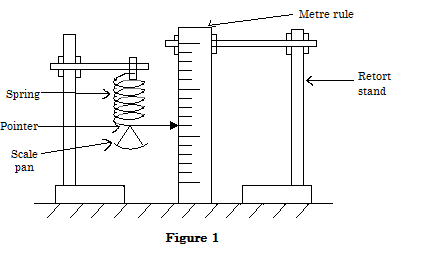
\includegraphics[width=14cm]{./img/2010-1-alt.png}
\end{center}

Set up the apparatus as shown in Figure 1. Put a mass of 50 g on the scale pan and record the equilibrium position $X_0$ of the pointer. Put on the scale pan the unknown weight marked $W$. Without removing $W$ and the 50 g mass in the scale pan, add a load $L$ of 50 g and record the new position of the pointer $X$. Calculate the extension $E = (X - X_0)$. Repeat this process for $L$ = 100 g, 150 g, 200 g and 250 g.
\begin{enumerate}
\item[(a)] Record you conclusions as shown in Table 1.\\[10pt]

Equilibrium position $X_0$..................\\[10pt]

Table 1\\[10pt]

%\begin{center}
\begin{tabular}{|p{3cm}|p{3cm}|p{3cm}|} \hline
\multicolumn{1}{|c|}{Load (g)} & \multicolumn{1}{c|}{$X$ (cm)} & \multicolumn{1}{c|}{$E = X - X_0$ (cm)} \\ \hline
\multicolumn{1}{|c|}{50} & & \\ \hline
\multicolumn{1}{|c|}{100} & & \\ \hline
\multicolumn{1}{|c|}{150} & & \\ \hline
\multicolumn{1}{|c|}{200} & & \\ \hline
\multicolumn{1}{|c|}{250} & & \\ \hline
\end{tabular}\\[10pt]
%\end{center}

\item[(b)] Plot the graph of load L against absolute value of extension E. The scale of the vertical axis should be chosen to range from 200 g to 300 g.
\item[(c)] From the graph, determine the unknown weight marked W, given that L = KE + W where K is a constant.
\item[(d)] What does the gradient of the graph represent?
\item[(e)] State the sources of errors and precautions that should be taken in the experiment.
\end{enumerate}
\end{enumerate}
\flushright \textbf{(25 marks)}

\pagebreak

\begin{enumerate}
\item[2.] The aim of this experiment is to determine the refractive index of water. Proceed as follows:

\begin{center}
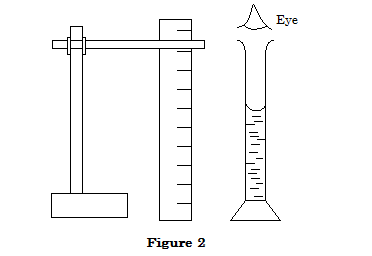
\includegraphics[width=10cm]{./img/2010-2-alt.png}
\end{center}

\begin{enumerate}
\item[(a)] Arrange your apparatus as in Figure 2. Put about 150 cm$^3$ of clear water in the measuring cylinder. Drop an office pin at the bottom so that it rests touching the wall of the cylinder.
\item[(b)] Look in the cylinder from Figure 2. Use another office pin as a search pin, move it up and down outside the cylinder, and locate the image position by no parallax method. Locate the image position of the ruler. Measure and record the depth ($H_1$) of the image. Measure and record the depth ($H_2$) of water. Repeat the experiment with 175 cm$^3$, 200 cm$^3$, 225 cm$^3$ and 250 cm$^3$ of water in the measuring cylinder.
\item[(c)] 
\begin{enumerate}
\item[(i)] Record in Table 2 your values of $H_1$ and $H_2$ corresponding to the volumes of water in the measuring cylinder.\\[10pt]

Table 2\\[10pt]

%\begin{center}
\begin{tabular}{|p{3cm}|p{3cm}|p{3cm}|} \hline
\multicolumn{1}{|c|}{Volume of water V (cm)} & \multicolumn{1}{c|}{$H_1$} & \multicolumn{1}{c|}{$H_2$} \\ \hline
\multicolumn{1}{|c|}{150} & & \\ \hline
\multicolumn{1}{|c|}{175} & & \\ \hline
\multicolumn{1}{|c|}{200} & & \\ \hline
\multicolumn{1}{|c|}{225} & & \\ \hline
\multicolumn{1}{|c|}{250} & & \\ \hline
\end{tabular}\\[10pt]
%\end{center}

\item[(ii)] Plot the graph of $H_2$ versus $H_1$.
\item[(iii)] Determine the slope of the graph.
\item[(iv)] What is the physical meaning of the slope?
\item[(v)] State sources of error in this experiment.
\end{enumerate}
\end{enumerate}
\end{enumerate}
\flushright \textbf{(25 marks)}

\pagebreak

\begin{enumerate}
\item[3.] The aim of this experiment is to determine the resistivity of an electrical conductor $P$.

\begin{center}
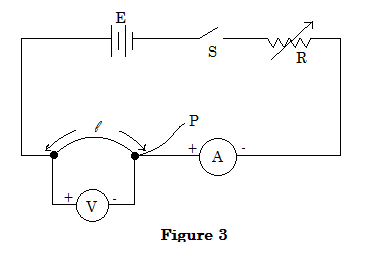
\includegraphics[width=10cm]{./img/2010-3-alt.png}
\end{center}

With $P$ having a length $l = 50$ cm, connect up the circuit as shown in Figure 3. Close one key S and adjust the rheostat R so that the current in $P$ is 0.20 A. Record the current $I$ and the potential difference $V$ between its ends.\\[10pt]

Repeat the procedure with current $I = $0.30 A, 0.40 A, 0.50 A and 0.60 A.
\begin{enumerate}
\item[(a)] Record your results in Table 3.\\[10pt]

Table 3\\[10pt]

%\begin{center}
\begin{tabular}{|p{3cm}|p{3cm}|} \hline
\multicolumn{1}{|c|}{Current $I$ (A)} & \multicolumn{1}{c|}{P.d. (volts)} \\ \hline
\multicolumn{1}{|c|}{0.20} &  \\ \hline
\multicolumn{1}{|c|}{0.30} &  \\ \hline
\multicolumn{1}{|c|}{0.40} &  \\ \hline
\multicolumn{1}{|c|}{0.50} &  \\ \hline
\multicolumn{1}{|c|}{0.60} &  \\ \hline
\end{tabular}\\[10pt]
%\end{center}

\item[(b)] Plot a graph of $V$ against $I$ and calculate the slope $G$.
\item[(c)] Deduce the resistivity of the conductor $P$ given that; $\rho = \cfrac{G\pi d^2}{4l}$.\\[10pt]
Where $\rho$ = resistivity\\
$d$ = diameter of $P$ (measured using the micrometer screw gauge provided).
\end{enumerate}
\end{enumerate}

\flushright \textbf{(25 marks)}
\flushleft